% !TeX root = ../main.tex
% Add the above to each chapter to make compiling the PDF easier in some editors.
\usetikzlibrary{positioning,fit,calc}

\chapter{Background}\label{chapter:background}

\section{Black Box Monitoring}

Black box monitoring is a well-established approach to system analysis, most commonly applied in software testing and network monitoring. It evaluates a system's functionality based on its responses to given inputs while abstracting away the system's internal workings~\parencite{jorgensenSoftwareTestingCraftsman2021}. This technique metaphorically views the system as a "black box" in ~\autoref{fig:example-black-box-monitoring}, signifying that the internal mechanisms are not visible or accounted for in the evaluation process~\parencite{myersArtSoftwareTesting2004}.

\begin{figure}[htpb]
    \centering
    % This should probably go into a file in figures/
    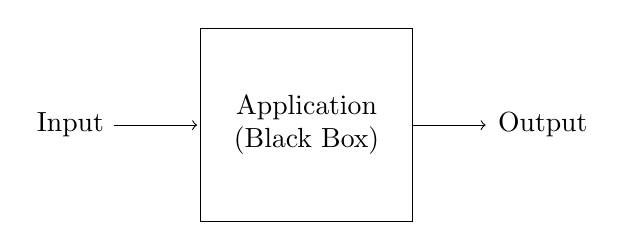
\begin{tikzpicture}[shorten >=1pt, node distance=3cm, auto]
      \node (R0) {Input};
      \node (R1) [right of=R0, minimum height=7em, text width=7em, align=center, draw] {Application\\(Black\ Box)};
      \node (R2) [right of=R1] {Output};
  
      \path[->]
        (R0) edge node {} (R1)
        (R1) edge node {} (R2);
    \end{tikzpicture}
    \caption[Example black-box monitoring]{An example of a black-box monitoring.}\label{fig:example-black-box-monitoring}
\end{figure}

One of the key advantages of black box monitoring is its simplicity and ease of implementation. Since it doesn't require in-depth knowledge of the system internals, it can be quickly deployed across various platforms and systems. This quality fosters wide applicability, accommodating diverse programming languages and system architectures. Furthermore, black box monitoring has a unique focus on the user experience. By simulating user actions and recording the system's responses, it offers a valuable measure of system functionality from a user's perspective. Thus, it is instrumental in ensuring that the system effectively meets the end-users' requirements~\parencite{nidhraBlackBoxWhite2012}. 

However, while the black box approach has its merits, it is not without challenges. One significant limitation is the potential for limited coverage. Since black box monitoring concentrates on the inputs and outputs, it might overlook internal system issues. If a problem doesn't immediately or directly affect the system output, it may remain undetected, only to potentially cause serious issues down the line~\parencite{spillnerSoftwareTestingFoundations2021}. Moreover, black box monitoring could contribute to inefficiency in troubleshooting. A system failure detected by black box testing can be difficult to diagnose and fix due to the lack of visibility into the system internals. Pinpointing the specific area of the system causing the issue may turn into a challenging endeavor.

Despite existing challenges, the prospects for black box monitoring are increasingly optimistic, particularly in our rapidly evolving digital landscape. As customer satisfaction and user experience become paramount in the digital economy, the ability of black box monitoring to accurately reflect system availability and performance from the user's perspective proves invaluable. Moreover, with the advancement of other evolving techniques like eBPF, the scope of black box monitoring continues to expand~\parencite{nevesDetailedBlackboxMonitoring2021}~\parencite{brondolinBlackboxMonitoringApproach2020}. For instance, eBPF's ability to execute custom code in kernel space can provide deeper insights into system operations, thereby enhancing internal observability~\parencite{jonathanBPFUniversalInkernel2014}.

As the IT landscape becomes more complex with microservices and cloud-based applications, understanding the internals of every service can be overwhelming. In such a scenario, black box monitoring's ability to provide a holistic view of system behavior can be highly beneficial. Moreover, in light of growing privacy regulations and data protection measures, black box monitoring's non-invasive approach aligns with the current trends. Focusing on system outputs rather than internals could potentially minimize privacy or data protection concerns.

In conclusion, black box monitoring remains a vital tool for system testing and monitoring, despite its inherent challenges. Its future appears increasingly integrated with AI technologies and aligned with user-centric design principles. Nevertheless, black box monitoring should not be considered a stand-alone solution but rather a component of a comprehensive monitoring strategy that incorporates various techniques to effectively manage system performance.

\section{Prometheus Agent and Blackbox Exporter}

The renowned Prometheus ecosystem provides two important components: the Prometheus Agent and the Blackbox Exporter. These technologies are extensively employed in various enterprises for monitoring applications in testing and production environments. Their widespread adoption is a testament to the reliability and robustness of the Prometheus platform in handling diverse monitoring needs.

The Prometheus Agent is a specialized mode of a standard Prometheus instance aimed at efficient data scraping and remote write as in ~\autoref{fig:prometheus-agent}. Unlike a full-fledged Prometheus server with functionalities like data storage and querying, the Prometheus Agent is streamlined for specific tasks, making it an ideal choice in distributed systems where resource optimization is crucial. This mode is invaluable when a full Prometheus server setup is unnecessary, facilitating a more streamlined and resource-efficient deployment. It is particularly effective in large-scale environments where managing the overhead and complexity of multiple complete Prometheus instances would be impractical~\parencite{prometheusIntroducingPrometheusAgent}.

\begin{figure}[htpb]
    \centering
    % This should probably go into a file in figures/
    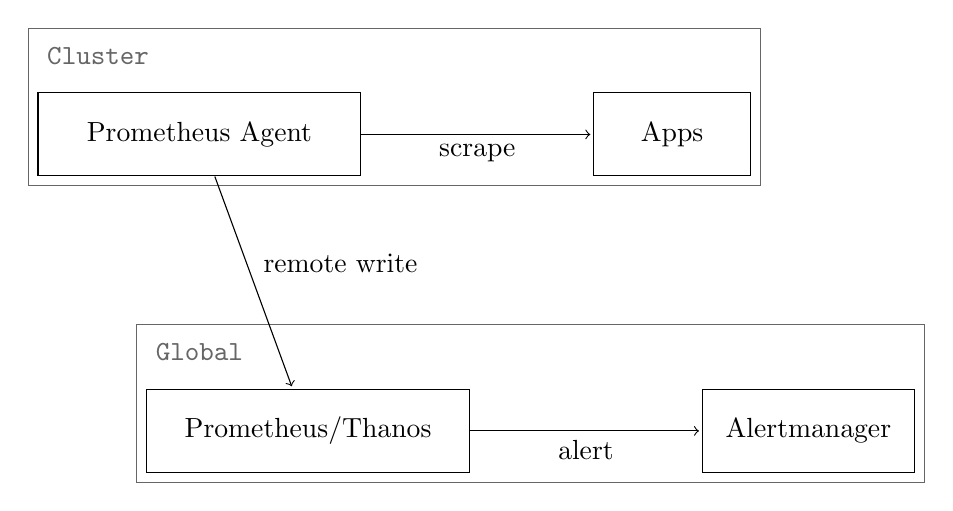
\begin{tikzpicture}[
        shorten >=1pt,
        zonetag/.style={align=center, font=\fontsize{10}{10}\color{black!60}\ttfamily},
        node/.style={draw, align=center, minimum height=3em, anchor=west}, 
        zone/.style={draw=black!60}
      ]

      \node (C) at(0, 0) [zonetag] {Cluster};
      \node (PA) [node distance=1cm, below=of C.west, text width=11em, node] {Prometheus\ Agent};
      \node (Apps) [node distance=5cm, right of=PA, text width=5em, node] {Apps};
      \node [zone, fit={(C) (PA) (Apps)}] {};

      \node (G) [node distance=2cm, below=of PA, zonetag] {Global};
      \node (P) [node distance=1cm, below=of G.west, text width=11em, node] {Prometheus/Thanos};
      \node (Am) [node distance=5cm, right of=P, text width=7em, node] {Alertmanager};
      \node [zone, fit={(G) (P) (Am)}] {};
  
      \path[->]
        (P) edge node[below, sloped] {alert} (Am)
        (PA) edge node[auto] {remote write} (P)
        (PA) edge node[below, sloped] {scrape} (Apps);
    \end{tikzpicture}
    \caption[Prometheus Agent]{Prometheus Agent with scrape and remote write.}\label{fig:prometheus-agent}
\end{figure}

The Blackbox Exporter, an essential element of the Prometheus toolkit, is designed to probe external endpoints across multiple protocols, including HTTP/HTTPS, TCP, and ICMP. This capability is fundamental to black box monitoring, enabling the assessment of system health and performance from an external viewpoint without necessitating internal access to the monitored system~\parencite{prometheusBlackboxExporter2023}. The Blackbox Exporter is instrumental in situations where internal monitoring is either not feasible or insufficient, such as in third-party services or in environments where internal metrics are not available or reliable.

Integrating the Prometheus Agent with the Blackbox Exporter fosters a distributed scheduler-executor architecture. This approach allows for a more granular and distributed monitoring framework, which is highly adaptable and can be effectively implemented across various platforms as service (PaaS) clusters with latencies~\parencite{prometheusUnderstandingUsingMultitarget}. Such an architecture bolsters the scalability and resilience of the monitoring system, rendering it suitable for large-scale and intricate environments. This distributed nature enhances the system's ability to scale and ensures a more resilient monitoring setup capable of withstanding node failures and network partitions~\parencite{prometheusIntroducingPrometheusAgent}.

Achieving optimal availability and scalability with the Prometheus Agent and Blackbox Exporter needs additional configuration and management. For the Prometheus Agent, employing relabeling is a crucial horizontal scaling or sharding strategy~\parencite{prometheusHowRelabelingPrometheus}. This method distributes the workload across multiple Prometheus Agent instances with a hidden label with hashed value, augmenting the system's capacity to handle substantial data volumes efficiently. Regarding the Blackbox Exporter, scalability is further enhanced by integrating a load balancer with properly configured scaling parameters, ensuring an even distribution of the probing load and maintaining system performance, even under high demand~\parencite{prometheusIntroducingPrometheusAgent}.

Overall, the active and extensive community surrounding Prometheus plays a significant role in the continuous improvement and reliability of the Prometheus Agent and Blackbox Exporter. This support ensures consistent updates and maintenance, effectively addressing the evolving needs and challenges in the monitoring domain. However, utilizing the Prometheus Agent and Blackbox Exporter to achieve scalability and manageability requires additional configurations and operations. Consequently, automating the scaling and management operations for both the Prometheus Agent and Blackbox Exporter emerges as a critical issue.

\section{Operator Pattern and Prometheus Operator}

The Operator Pattern, defined by the \ac{CNCF}, represents a paradigm shift in Kubernetes, enabling users to automate the maintenance and configuration of applications~\parencite{kubernetesOperatorPattern}. The Prometheus Operator embodies this pattern, serving as an implementation that addresses the practical needs of deploying and managing Prometheus components. Through reconciliation, the Prometheus Operator aligns the deployment's actual state with the user's desired state, streamlining its lifecycle in Kubernetes~\parencite{prometheusoperatorIntroduction2020}.

The Operator Pattern extends Kubernetes' native capabilities by introducing \ac{CRs} and controllers. The operator is the essential software extension that utilize the Kubernetes control plane and API to create, configure, and manage instances of complex stateful applications on behalf of a Kubernetes user~\parencite{dobiesKubernetesOperators}. They encapsulate operational knowledge, automating the management tasks that would typically require manual operations~\parencite{cncfCNCFOperatorWhite}. 

The Prometheus Operator is tailored to simplify the deployment and management of Prometheus within Kubernetes environments. It enables Kubernetes-native deployment and automated management of Prometheus and its associated monitoring components. Key features of the operator include Kubernetes \ac{CRs} for deploying and managing Prometheus, Alertmanager, and so on, streamlined deployment configurations for setting up Prometheus essentials like versions and retention policies, and automatic generation of monitoring target configurations. This approach facilitates easy installation and version upgrades, simplifies configuration management, and ensures seamless integration with existing Kubernetes resources~\parencite{prometheusoperatorIntroduction2020}. 

In terms of current advancements in black box monitoring, the Prometheus Operator supports two \ac{CRs}: Probe and PrometheusAgent. The Probe resource defines monitoring for a set of static targets or ingresses, such as specifying the target for the Blackbox Exporter and the module to be used. On the other hand, PrometheusAgent is responsible for defining a Prometheus agent deployment. This includes configurations like the number of replicas, ScrapeConfigs, and advanced features like sharding~\parencite{prometheusoperatorPrometheusAgentSupport}. Notably, it incorporates the ProbeSelector feature, which links to the previously defined Probe resource, enhancing its functionality and integration~\parencite{prometheusoperatorAPIReference}.

Despite these advancements, a significant gap persists in the management and configuration of the Blackbox Exporter within the Prometheus Operator framework. Specifically, there is no support for using a custom resource definition to manage the Blackbox Exporter. Consequently, users are required to deploy their own instances and modules of the Blackbox Exporter~\parencite{prometheusBlackboxExporter2023}. This limitation underscores the need for more integrated solutions that can simplify the deployment and scaling of the Blackbox Exporter, ensuring it meets the evolving requirements of black box monitoring in complex environments. 

In conclusion, while the Prometheus Operator has made significant strides in enhancing the ease and efficiency of deploying Prometheus in Kubernetes environments, there is still room for improvement, particularly in the realm of black box monitoring. Addressing the current limitations in the management of the Blackbox Exporter will be crucial in realizing the full potential of Prometheus as a comprehensive monitoring solution. 